\chapter{Revisão bibliográfica}
\label{Cap:RevisaoBibliografica}
\newcommand{\WidthAlgumaCoisa}{6.5 cm}


% Capítulo 2: Revisão Bibliográfica

\section{Tecnologia de Monitoramento de Ônibus}

\indent
\par De acordo com a informação exposta em uma publicação feita em 2017 pela Escola de Negócios da Universidade de Indiana, era previsto um crescimento anual de mais de 23\% no mercado de \textit{Big Data} durante o período de 2014 a 2019, com um custo de \$48,6 bilhões no último ano. Isso inclui um crescimento de 30\% entre 2014 e 2015 de aparelhos conectados e dispositivos de IoT. Estes aparelhos geram uma quantidade enorme de dados valiosos para quem tiver interesse de processá-los \cite{Lee2017}. Esse cenário hoje não é diferente para o setor de transporte público, com a prefeitura de São Paulo capturando dados em tempo real da sua frota de ônibus, informações como bilhetagem, velocidade e paradas dos veículos, porém não utilizando a informação para a tomada de decisão.

\par Um exemplo de uso prático desses dados foi apresentado na Conferência Internacional da Logística e Transporte Avançado. Em uma colaboração entre a IBM e o Conselho da Cidade de Dublin foi realizado um projeto de cidade inteligente entre 2010 e 2013 \cite{BenAyed2015}. A IBM passou a processar os dados gerados pela frota de ônibus, além de outras fontes, com intenção de reduzir o trânsito na cidade sem precisar alterar a sua estrutura atual, que conta com vários pontos históricos. O inicio do processo se dava com informações coletadas do ônibus, como dados de GPS, velocidade, paradas e bilhetagem, e depois eram adicionadas novas informações vindas de sistemas de semáforos, \textit{CCTV}, sistemas meteorológicos, entre outros. Todos esses dados então eram processados em um servidor da IBM e disponibilizados em mapa em tempo real do transporte público de Dublin. Com toda essa informação processada, a cidade teve uma maior capacidade de monitorar o seu sistema de transporte público, diminuindo o tempo para uma tomada de decisão.

\par Outro exemplo de aplicação de tecnologia no monitoramento de transporte coletivo é do USapiens, um sistema desenvolvido por um time de pesquisa da IBM do Brasil \cite{Vieira2015}. Essa equipe usou dados de transporte coletivo da cidade do Rio de Janeiro para desenvolver um sistema que processa os dados recebidos pelo GPS dos ônibus e depois disso analisa-se por diversos modelos esses dados. Para isso eles integraram os dados obtidos pelo GPS com informações disponíveis de GTFS \cite{GTFS}, sigla para \textit{General Transit Feed Specification}, que contém dados mais gerais das rotas de ônibus, como paradas e horários esperados. Feita essa integração, os dados são limpos para prevenir problemas como latitude/longitude imprecisas ou dados com intervalo de tempo muito grande. Com os dados prontos, é feita uma comparação com a rota do GTFS, se descobre a direção do veículo e com isso tem seu trajeto normalizado em uma escala de distância e tempo acumulativas.

\par Com a informação normalizada, o sistema pode ajudar a responder três perguntas principais. Através de uma análise descritiva histórica podemos responder "O que aconteceu e porque?", analisando os dados em tempo real se responde "O que está acontecendo e porque?" e uma análise preditiva responde "O que vai acontecer e porquê?". Os pesquisadores da IBM depois aplicaram esse sistema a 5 casos de estudo. O primeiro foi uma Análise de Uniformidade dos Ônibus, para evitar um agrupamento de veículos na linha, o segundo caso foi uma verificação na rotas dos ônibus, para avaliar a aderência do veículo a sua rota pré-definida, o terceiro uma análise de fluxo no trânsito, o quarto a variância do tempo de viagem do veículo, que permite avaliar a consistência da rota analisada, e para o quinto ele usaram a análise preditiva para prever o tempo de chegada do ônibus.

\section{\textit{Dashboard}}

\indent
\par O \textit{Dashboard}, também chamado de painel de controle, é uma ferramenta que auxilia os gestores a terem uma visão mais sistemática das principais informações do negócio. Em outras palavras, é um recurso que visa consolidar os dados de maior relevância em um painel, facilitando o processo de análise e a tomada de decisão \cite{Intelipost}.

\par O uso de planilhas e relatórios já são ultrapassados para análises de dados, não sendo suficientes para suprir as necessidades mais urgentes. Conforme a tecnologia foi evoluindo no mundo corporativo, surgiram os \textit{dashboards} que evitam esforços desnecessários e ter uma visão mais ampla de todo o cenário corporativo para, assim, tomar decisões estratégicas e assertivas.

\par A visualização de dados através de \textit{dashboards} já é uma realidade em softwares de gestão empresarial, integrando painéis de controle com inteligência artificial e fornecendo informações atualizadas automaticamente. É possível personalizá-los e comparar dados através de filtros, que facilitam análises de indicadores \cite{Tecnicon}.


\subsection{Uma ferramenta de apoio à decisão}

\indent
\par Segundo um estudo feito pela UNINDU (The International Congress on University Industry), 83\% das pessoas absorvem melhor as informações através da visão. Isso demonstra a importância do \textit{dashboard} para tomada de decisões rápidas e melhor análise dos indicadores,melhorando metas e atingindo objetivos.
\par O \textit{Business Intelligence} (BI) \cite{TableauBI}, por exemplo, é uma área que exige precisão na coleta e controle das informações para gerar insights em base desta ferramenta. Os dados são agrupados em conjuntos de registros e disponibilizadas por meio de \textit{dashboards} para mensurar o desempenho atual e futuro da empresa de acordo com o cenário.
\par Além disso, os \textit{dashboards} monitoram os dados, com o intuito de melhorar todos os processos. Eles permitem que o usuário personalize painéis e filtre informações para a visualização dos resultados, como quantidade, tempo e outras opções \cite{Tecnicon}.
\par A aplicação dos \textit{dashboards} na gestão empresarial traz muitos benefícios para a tomada de decisão e a visão estratégica do seu negócio, que fica cada vez mais fácil através da centralização,  visualização e compreensão das informações, o que possibilita uma visão ampla do seu negócio. Na gestão, é importante que todas as equipes tenham acesso aos indicadores da empresa, mantendo a transparência das informações. As ferramentas de \textit{dashboard} tem o objetivo de facilitar a comunicação interna entre todos os profissionais, otimizando o tempo para tomarem decisões e evitarem trabalhos manuais e complexos com a organização de dados, passando a priorizar outras atividades mais relevantes. Com as informações consolidadas em um único painel, a gestão se torna mais ágil e efetiva, possibilitando o alinhamento de estratégias e decisões para o negócio \cite{Tecnicon}.
\par Como o \textit{dashboard} trabalha com atualizações constantes e análises mais específicas, é mais fácil prever problemas e tendências negativas que podem vir a acontecer. Estes problemas ficam mais explícitos com o uso da tecnologia de inteligência artificial que os identifica de maneira mais fácil.
\par Qualquer mudança é detectada com mais simplicidade e o tempo para pensar nas possíveis soluções se torna muito maior. Isso melhora o processo de tomada de decisão e evita possíveis prejuízos \cite{Systemsat}.
\par Uma boa interface e uma boa experiência de uso se dá pela arquitetura das informação do \textit{dashboard}. É fundamental que seja organizado, coerente e intuitivo. O objetivo é tornar o mais fácil possível encontrar o que se procura. Através de menus, cores e  símbolos é possível saber quais são as opções e deixar claro as consequências que cada ação irá gerar. Dessa forma, a experiência do usuário ao usar o \textit{dashboard} será rápida e efetiva, atendendo suas expectativas \cite{Hostinger}.

\section{Desenvolvimento \textit{web} com Django}

\indent
\par Django é um \textit{framework web} de alto nível, escrito em Python que encoraja o desenvolvimento rápido, limpo e pragmático de aplicações \textit{web} \cite{Django}. Com ele é possível que o desenvolvedor se preocupe mais com as regras de negócio do que com a programação em si, uma vez que ele já implementa tratamento de requisições, mapeamento objeto-relacional, preparação de respostas HTTP, sistema de autenticação, entre outros. Além disso, o Django foi desenvolvido com um foco extra em segurança, implementando camadas que evitam os ataques mais comuns conhecidos.
\par A arquitetura do Django se baseia no padrão MTV (\textit{Model-Template-View}) \cite{MTV}, que por sua vez é bem parecido com o padrão MVC (\textit{Model-View-Controller}) \cite{MVC}, mas possui suas peculiaridades. Primeiramente, a camada conhecida como \textit{Model} é a responsável pelo mapeamento do banco de dados para o projeto. A camada \textit{Template} é a responsável pelo \textit{layout} da página, ou seja, como os dados serão exibidos para o usuário. Por fim, na \textit{View} é onde o processamento dos dados irá ocorrer antes de serem exibidos e onde ficam localizadas as regras de negócio.
\par Devido a essa arquitetura utilizada por padrão no Django, cada projeto é subdividido em diversos aplicativos, que são criados conforme a necessidade do desenvolvedor, os quais implementam individualmente o modelo MTV. Isso permite que esses aplicativos se tornem partes independentes do sistema, aumentando a sua portabilidade para outros projetos e consequentemente, o reaproveitamento de código.
\par Assim sendo, um aplicativo Django criado por algum desenvolvedor pode ser facilmente transformado em um pacote Python e disponibilizadao no repositório de \textit{softwares} oficial do Python, o PyPI \cite{PYPI}. Isso permite que a comunidade reutilize um mesmo código que já foi desenvolvido para uma finalidade específica. Dois importantes pacotes utilizados neste projeto são o Django REST \textit{Framework} \cite{DjangoRF}, que permite a fácil criação de APIs integradas com os modelos do Django e o Django \textit{Plotly Dash} \cite{DjangoPD}, que implementa múltiplos estilos de gráficos e visualizações de dados escrevendo apenas código Python, que por sua vez podem ser facilmente incluídos em um template do Django.

\section{Agendamento e execução de tarefas com Celery}

\indent 
\par O Celery é um sistema em Python simples, flexível e confiável para processar grandes quantidades de mensagens ou tarefas \cite{Celery}. Além disso é fácil de integrar com sistemas \textit{web}. Ele permite a delegação de tarefas a diversos \textit{workers}, localizados em outros servidores, ou seja, as tarefas são processadas de forma apartada da aplicação. De forma automática é criada uma fila de tarefas com foco no processamento em tempo real, ao mesmo tempo que oferece suporte ao agendamento de tarefas. É importante salientar que o Celery pode ser divididos em alguns componentes tais quais aplicação, \textit{broker}, \textit{worker} e \textit{beat}.
\indent 
\par A aplicação se refere ao próprio projeto ao qual o Celery vai ser implementado. Nela é necessário que existam funções ao qual devem ser executadas de forma apartada. Isso auxilia no desempenho principal do projeto.
\indent 
\par O \textit{broker} se refere ao sistema de gerenciamento de filas responsável por gerenciar todo o sistema de envio de tarefas, seja de forma assíncrona ou não. Existem várias opções para escolha de \textit{broker} como RabbitMQ, Redis, Amazon SQS, Zookeeper. Dependendo do sistema operacional ou do local onde o projeto funcionará verifica-se a melhor opção. Neste projeto, como foi utilizado o sistema de nuvem da Amazon (AWS), foi escolhido o SQS, pois trata-se de um serviço oferecido pelo própria AWS.
\indent 
\par O \textit{worker} é quem executa de fato as tarefas agendadas e enviadas pela aplicação no \textit{broker}. É nele que todo o processamento de execução fica. Existem algumas opções de execução que podem ser configuradas dependendo da necessidade do projeto. Dentre elas estão \textit{prefork}, \textit{solo}, \textit{eventlet} e \textit{gevent}. Basicamente o \textit{prefork} e o \textit{solo} trabalham de forma síncrona e utiliza consideravelmente a CPU por travá-la enquanto a solicitação não termina até começar a próxima. Por outro lado, o \textit{eventlet} e o \textit{gevent} funcionam de forma assíncrona e são mais indicados para requisições HTTP pois levam em conta o tempo de resposta do servidor e não consomem a CPU \cite{CeleryEP}. 
\begin{figure}[H]
    \centering
    \caption{Diagrama de funcionamento do Celery}
    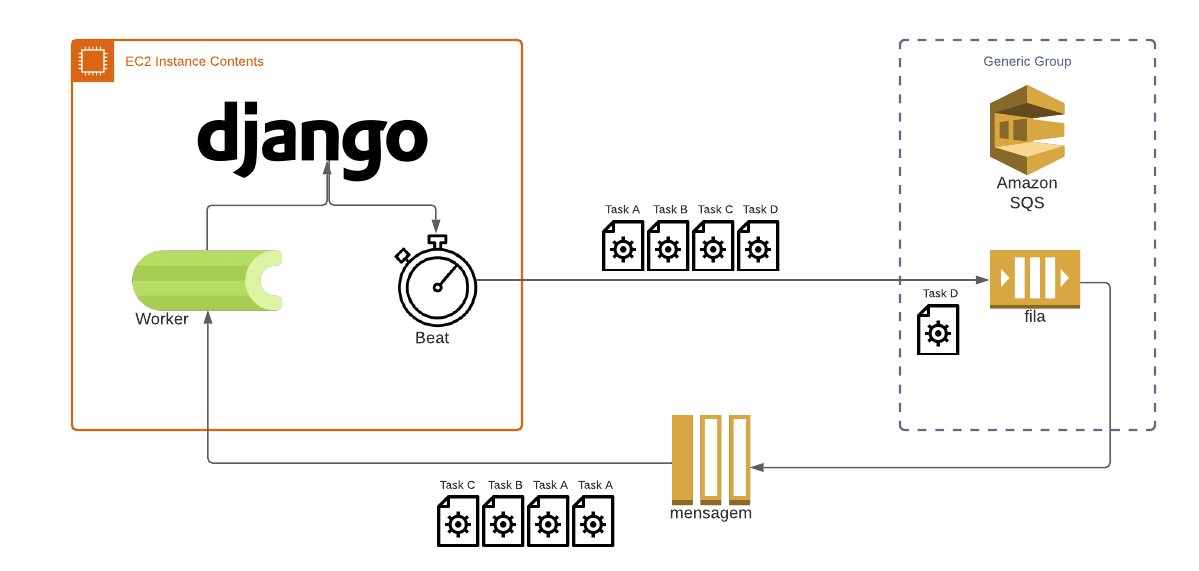
\includegraphics[width=1.0\linewidth]{Imagens/diagramaCelery.png}
    \caption*{Fonte: Arquivo dos autores (2020)}
    \label{DiagramaDeBlocosIcones}
\end{figure}
\indent 
\par O \textit{beat} é um componente opcional que que dispara de tempos em tempos as tarefas para o \textit{broker}, como se fosse a aplicação. No projeto decidimos utilizá-lo pois é preciso que de tempos em tempos, de forma programada, uma tarefa seja executada de forma assíncrona \cite{CeleryTAP}.

\section{Computação em Nuvem}

\indent
\par Eric Knorr, editor chefe da InfoWorld, dá dois significados para a expressão Computação em Nuvem \cite{CloudComp}, o primeiro, e mais comum, refere-se a serviços que executam processos remotamente, em servidores de empresas que provém esse tipo de serviço, como a Amazon Web Services, Microsoft Azure e Google Cloud Platform. O segundo significado é a descrição de como esses serviços funcionam, um conjunto de recursos computacionais disponíveis sob demanda. 
\indent
\par Essas infraestruturas permitem seus clientes usarem os recursos de maneira escalável e instantânea, sem precisar se preocupar com a infraestrutura física ou com a necessidade de \textit{softwares} novos. As empresas provedoras garantem a manutenção das máquinas em si e permitem que os usuários foquem no serviço que estão prestando ou desenvolvendo.
\indent
\par Entre os serviços que esse modelo de computação fornece estão o SaaS, \textit{software} como serviço ou \textit{software} as a \textit{service}, que são as aplicações que acessamos pelo navegador, como o Google Suit ou o Office 365, o IaaS, infraestrutura como serviço ou \textit{infrastructure as a service}, que são soluções completas de computação na nuvem, permitindo desde de máquinas virtuais simples até servidores que precisam atender grandes demandas de processamento a todo momento, o PaaS, plataforma como serviço ou \textit{platform} as a service, que são serviços com plataformas já minimamente configuradas, voltadas a desenvolvedores que precisam de agilidade para disponibilizar uma aplicação e que não querem ter o trabalho de configurar um IaaS mais completa, e por último o FaaS, função como serviço ou \textit{function as a service}, que é uma camada de abstração do PaaS, onde o desenvolvedor precisa de apenas alguns trechos de código para se comunicar com funções específicas do seu provedor de nuvem, como AWS Lambda ou o IBM OpenWhisk \cite{CloudComp}.

\subsection{Amazon Web Services}

\indent
\par Em 2006 a gigante do varejo eletrônico Amazon decidiu disponibilizar e rentabilizar a sua infraestrutura de TI, tecnologia da informação, para outros usuários através de um serviço, o Amazon Web Services, ou simplesmente AWS \cite{AmazonAWSAbout}. Hoje esse serviço gera uma renda anual de mais de 35 bilhões de dólares \cite{DevelpAmazonWeb} e atende mais de 1 milhão de usuários, incluindo empresas como Johnson \& Johnson, McDonald\'s e Samsung \cite{WhosUsingAWS}.
\indent
\par Hoje, a AWS, oferece mais de 175 serviços diferentes, partindo de armazenamento de dados até ferramentas para IoT \cite{TopTenAWS}. Seus principais serviços incluem o \textit{Elastic Compute Cloud} (EC2), o \textit{Simple Storage Service} (S3) e o AWS Lambda \cite{TechRadar}.

\subsubsection{Elastic Compute Cloud}

\indent
\par Jeff Barr, atual vice presidente da AWS, anunciou em agosto de 2006 o lançamento da versão de testes do \textit{Elastic Compute Cloud} \cite{AWSEC2Beta}, que se tornaria o principal recurso dentro das opções oferecidas pela AWS. Inicialmente oferecendo um sistema com um processador Intel Xeon de 1,7 GHz, 1,75 GB de RAM, 160 GB de disco rígido e uma conexão de 260 Mb/s, tinha o custo de 10 centavos de dólar por hora, podendo executar distribuições de Linux, e já contava com um alto nível de escalabilidade, com o usuário tendo a possibilidade de executar quantos sistemas, chamados de "\textit{virtual CPU}", ele achasse necessário.
\indent
\par Hoje o EC2 suporta várias distribuições de Linux, incluindo Red Hat Enterprise, Ubuntu e a distribuição própria da Amazon, o Amazon Linux, Windows Server e Raspbian para seus servidores com plataforma ARM \cite{awsSuppSystems}. Além disso, também é possível escolher várias configurações de hardware em várias faixas de preço partindo de versões básicas, com apenas um núcleo e 1 GB de RAM, sem custo, até máquinas com múltiplos processadores físicos e múltiplas GPUs, que cobram mais de 10 dólares a hora, ficando a cargo do usuário escolher a opção que o melhor atende \cite{AWSINSTANCE}.

\subsubsection{Simple Queue Service}

\indent
\par O \textit{Simple Queue Service} (SQS) é um dos serviços web mais antigos fornecido pela Amazon, sendo anterior até mesmo a AWS. Lançado em 2004 \cite{JeffBarr}, ele fornece uma API genérica para ser usada em gerenciamentos de fila em linguagens suportadas pelo AWS SDK, por meio de mensagens armazenadas e enviadas pelo servidor.
\indent
\par As vantagens de usar um serviço como o SQS no lugar de soluções locais, como Redis ou o RabbitMQ, é a disponibilidade e a escalabilidade que um serviço como a AWS fornece. Por meio de redundância de servidores a AWS garante que o SQS estará sempre disponível para processar e consumir as mensagens e poderá escalar o seu serviço caso receba uma carga muito grande dessas chamadas \cite{AWSSQS}.

\subsubsection{Relational Database Service}

\indent
\par O AWS \textit{Relational Database Service}, ou simplesmente RDS, é um serviço de banco de dados pré configurado, em que o usuário interage através de uma API em não tem o trabalho de configurar uma instância apenas para o seu banco de dados e também não precisa se preocupar com o uso de recursos da infraestrutura onde a sua aplicação principal está sendo executada, seja em uma instância EC2, um serviço como o AWS Lambda ou um servidor local \cite{AWSRDS_B}.
\par Lançado em 2009 com suporte apenas a MySQL, hoje o serviço pode executar vários tipos de banco de dados relacionais, como MariaDB, PostgreSQL e Oracle \cite{AWSRDS}. Por funcionar como uma abstração de uma instância EC2, o RDS oferece as mesmas vantagens, incluindo um alto nível de escalabilidade, o que permite que seja usado por grandes empresas como Netflix, Expedia e Unilever.

\subsection{Google Cloud Platform}

\indent
\par A Google tem uma plataforma que concorre com a AWS, a Google Cloud Platform (GCP), que a apesar de oferecer serviços como o Google \textit{Cloud Engine} e o Google \textit{Cloud Storage}, equivalentes ao AWS EC2 e AWS S3, tem um foco maior em containers e serviços próprios da Google, como o Google Maps e o Google Suit \cite{ZdNet}.
\indent
\par Através da GCP é possível fazer consultas por API ao Google Maps, o que permite consultas de endereços partindo do nome de locais ou mesmo o uso de mapas completos adaptados a necessidade da aplicação \cite{GMP}.

\section{Análise de Dados}

\indent
\par Apesar de estar cada vez mais em destaque nestes últimos anos, podemos traçar o uso de estatística para tomada de decisão desde do Egito Antigo, de acordo com um artigo publicado por Keith D. Foote \cite{Foote2018} os egípcios já usavam cálculos estatísticos para construir as pirâmides. Já na década de 1880, o governo americano levou pelo menos 7 anos para completar o censo da população, processo que foi reduzido para um ano e meio na década seguinte por causa do desenvolvimento de uma máquina de tabulação, por Herman Hollerith, que processava os dados de forma sistêmica em cartões perfurados.

\subsection{Fases da análise de dados}

\indent
\par Trazendo para os dias atuais, a Universidade de Villanova separa a análise de dados em três estágios. O primeiro deles seria o início do que chamamos de \textit{Business Intelligence}, que surgiu por volta de 1950 como uma forma de processar pequenas quantidades de informações estruturadas. Esse estágio, que podemos chamar de \textit{Analytics 1.0}, durou até cerca de 2009, quando foi consolidado o termo \textit{"big-data"}.
\par O fim do primeiro estágio se deu pelo aumento exponencial de dados sendo produzidos diariamente, podendo vir de qualquer lugar e forma, desde de informações simples e estruturadas, como quais produtos alguém comprou em um determinado site, ou coisas mais complexas, como quais sites fizeram essa pessoa chegar até uma determinada página e qual a posição geográfica dessa pessoa quando acessou a página. Se convencionou a chamar esses dados em grande quantidade e pouco estruturados de \textit{"big-data"}.
\par Pela dificuldade de armazenar e processar essa massiva quantidade de dados, se fez necessário o desenvolvimento de novos métodos e ferramentas para o processamento deles, o que deu início ao \textit{Analytics 2.0}, que trouxe alternativas como Hadoop, que pode processar essas grandes massas de dados, e o NoSQL, que permite armazenar toda a informação de forma mais eficiente que os bancos de dados relacionais faziam até então. Além disso, cada vez mais se fez necessário um conhecimento tecnológico para fazer essas análises, quando até então bastava o conhecimento de métodos estatísticos.
\par Hoje em dia, muitos especialistas dizem que chegamos a um terceiro estágio, o \textit{Analytics 3.0}, onde esses dados que são produzidos a qualquer momento podem ser usados como moeda de troca entre consumidor e fornecedor. Essa moeda pode ser analisada imediatamente pelo fornecedor, que passa a entregar uma experiência personalizada para quem está consumindo o seu produto \cite{Villanova}.

\subsection{Análise de dados no dia a dia}

\indent
\par Com a disponibilidade de dados que temos, as empresas estão se dedicando cada vez mais em coletar e auxiliar as suas decisões nas análises feitas com eles. O Diretor de Estratégia e Marketing de Precisão da Coca-Cola, Justin De Graaf, afirmou em entrevista para ADMA, Association for Data-Driven Marketing \& Advertising, que cada vez mais a empresa usa informações coletadas diretamente dos consumidores, como por meio de telefone, redes sociais ou \textit{e-mail}, para criar desde campanhas publicitárias até novos produtos \cite{Tan2017}. Outra marca consolidada usando análise de dados para a tomada de decisão é a rede de hotéis Marriott, que, de acordo com o seu \textit{chief development officer}, Eric Jacobs, tem usado esse tipo de informação para decidir como identificar, atrair e manter os seus cliente mais lucrativos \cite{Eisen2018}. Para isso eles coletam desde dados como padrão social dos clientes até se eles consomem mais jeans Levi's ou Gap.

\par Apesar disso, alguns resultados dessas análises podem ter um efeito contrário do que era pretendido no início. Caso a análise não seja feita com atenção, verificando sempre quem está sendo atingido, ela pode levar a alguns atritos e desgastar a imagem de quem usa essas informações.

\par Em 2012, o New York Time publicou uma história de como um pai descobriu a gravidez da filha através de uma promoção oferecida pela rede varejista Target, nos Estados Unidos \cite{Duhigg2012}. Andrew Pole, um estatístico da rede, foi designado para desenvolver um "preditor de gravidez", no fim do estudo ele conseguiu chegar a uma lista de 25 produtos, que geram uma probabilidade da cliente estar grávida de acordo com o seu preditor. Esses produtos contêm itens como manteiga de cacau, bolsas grandes o suficiente para caber pacotes de fraldas, e suplementos como magnésio e zinco.

\par A Target vinculava essa informação a um identificador do cliente, e então ofereceria um desconto na próxima visita que essa mesma pessoa fizesse a loja. Um ano após a aplicação deste preditor, o pai de uma adolescente foi a uma das lojas reclamar que sua filha tinha recebido um desconto relacionado a esse programa específico para grávidas, com isso, o gerente da loja se desculpou pelo erro e alguns dias depois ligou para se desculpar novamente. Entretanto, para a surpresa do gerente, durante essa ligação o cliente disse que a filha não tinha contado para ele que estava grávida, e que a Target soube antes dele do acontecido. Após esse caso, o departamento de \textit{marketing} decidiu desacelerar o programa de análises de dados, e passar mais tempo avaliando qual impacto cada iniciativa pode ter.
